\section{Experimento 2: Red hogareña}

\subsection{Descripción del contexto}

El experimento fue realizado en una red doméstica, por medio de una conexión Wi-Fi de Fibertel.
Al momento de tomar las mediciones estaban conectados a la red una laptop, una smart TV, un celular y una tablet. 
La fecha de la captura fue Sábado 7 de Octubre de 2017. 

Adicionalmente, el celular estaba tambien siendo usado como control remoto por el programa VLC.

\subsection{Descripción de la captura}

%% distribucion de protocolos (grafico)
La captura resulto en un trafico de 10000 paquetes en total. 
La figura 6 muestra la distribución de protocolos dentro de la captura. 
Observamos paquetes de tipo IPv4, IPv6(0x86dd ), ARP y también Fast Roaming Internet Request. Este último es un protocolo usado en redes inalambricas, especificamente con dispositivos mobiles en movimiento como son los celulares.
\begin{figure}[H]
\centering
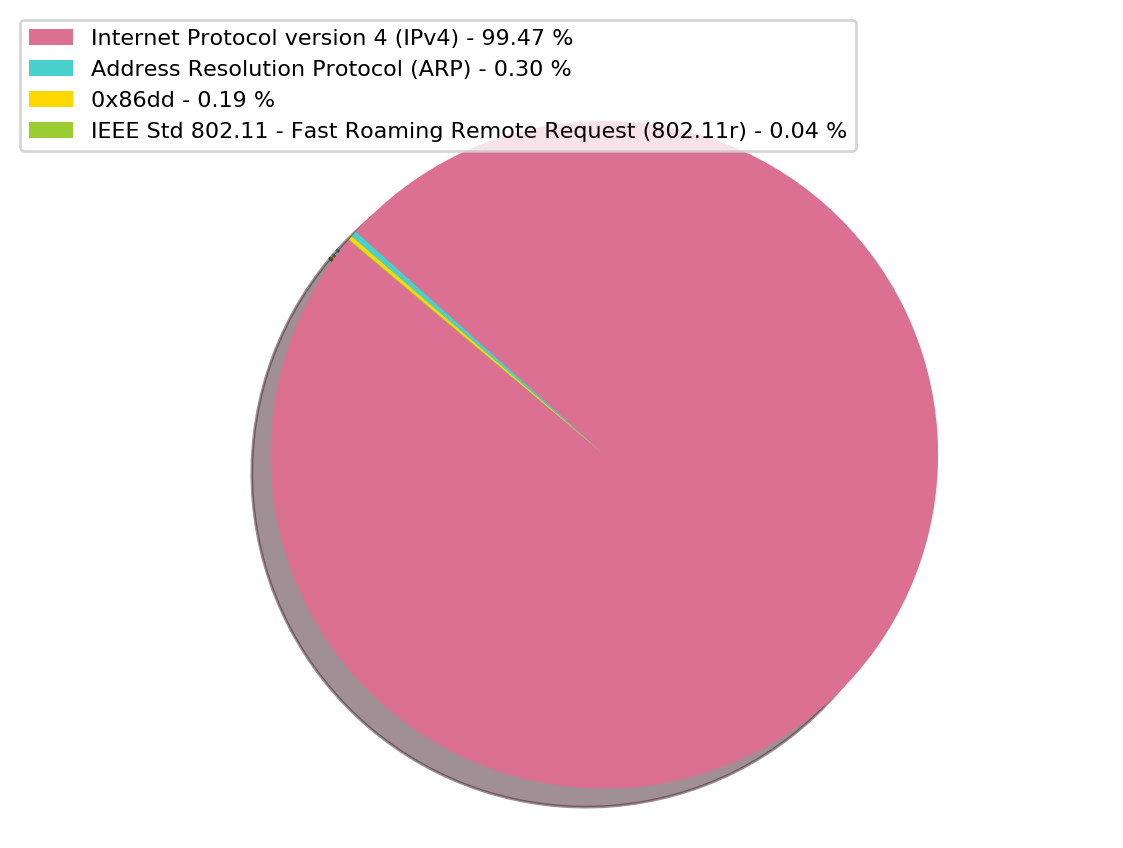
\includegraphics[width=0.7\textwidth]{protocolosRed2.png}
\caption{Gráfico que muestra la distribución de protocolos en la red.}
\label{broadcast2}
\end{figure}

En la figura 7 podemos ver el porcentaje de paquetes broadcast sobre el total de paquetes capturados. 
Vemos que representan un 1,8% del total. 

En la figura 8 vemos que los protocolos que presentan paquetes de tipo broadcast son ARP e IPv4. 
El porcentaje de broadcast es mucho menor al de la primer red. Atribuimos esto al hehco de que hay menos dispositivos en uso conectados a la red.

%% grafico de broadcast
\begin{figure}[H]
\centering
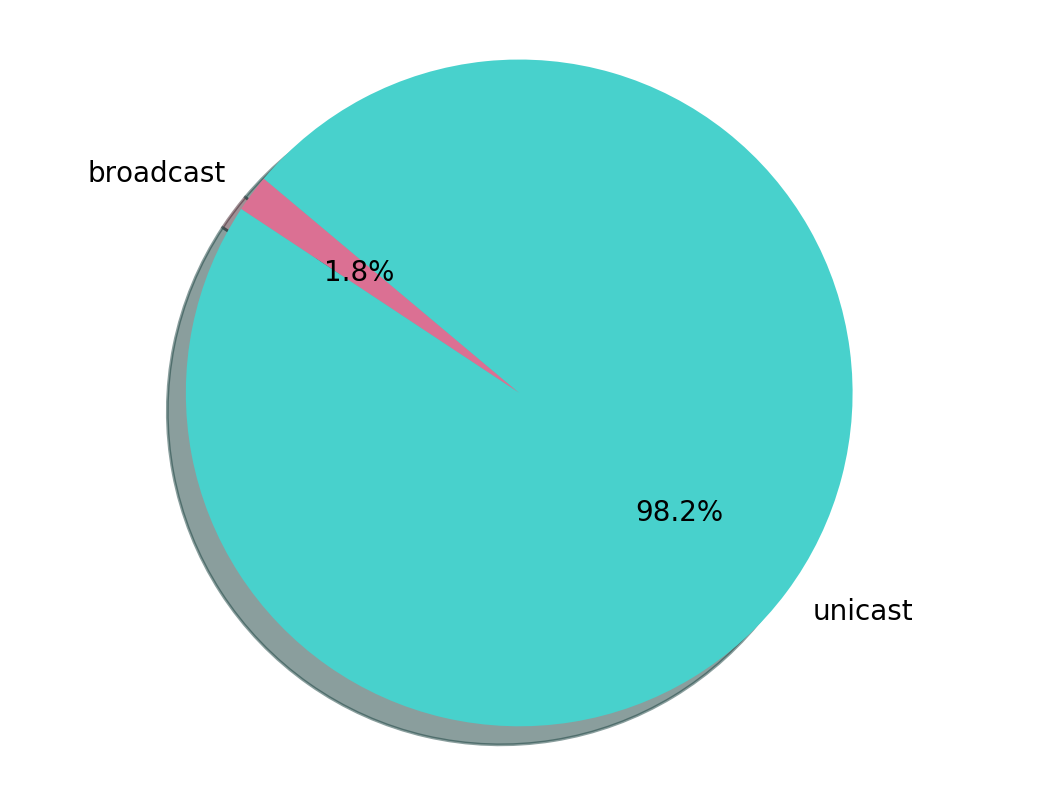
\includegraphics[width=0.7\textwidth]{broadcastRed2.png}
\caption{Gráfico que muestra los porcentajes de tráfico broadcast y unicast.}
\label{broadcast2}
\end{figure}

\subsection{Análisis de la captura}

La figura~\ref{entropias1_2} muestra la información de cada símbolo de la fuente S1 para esta red. 
Observamos que hay un símbolo cuya información es disitntivaente mas baja en comparación con la de los demás (IPv4 unicast); lo cual  hace que la entropía muestral sea mucho menor a la máxima.

\begin{figure}[H]
\centering
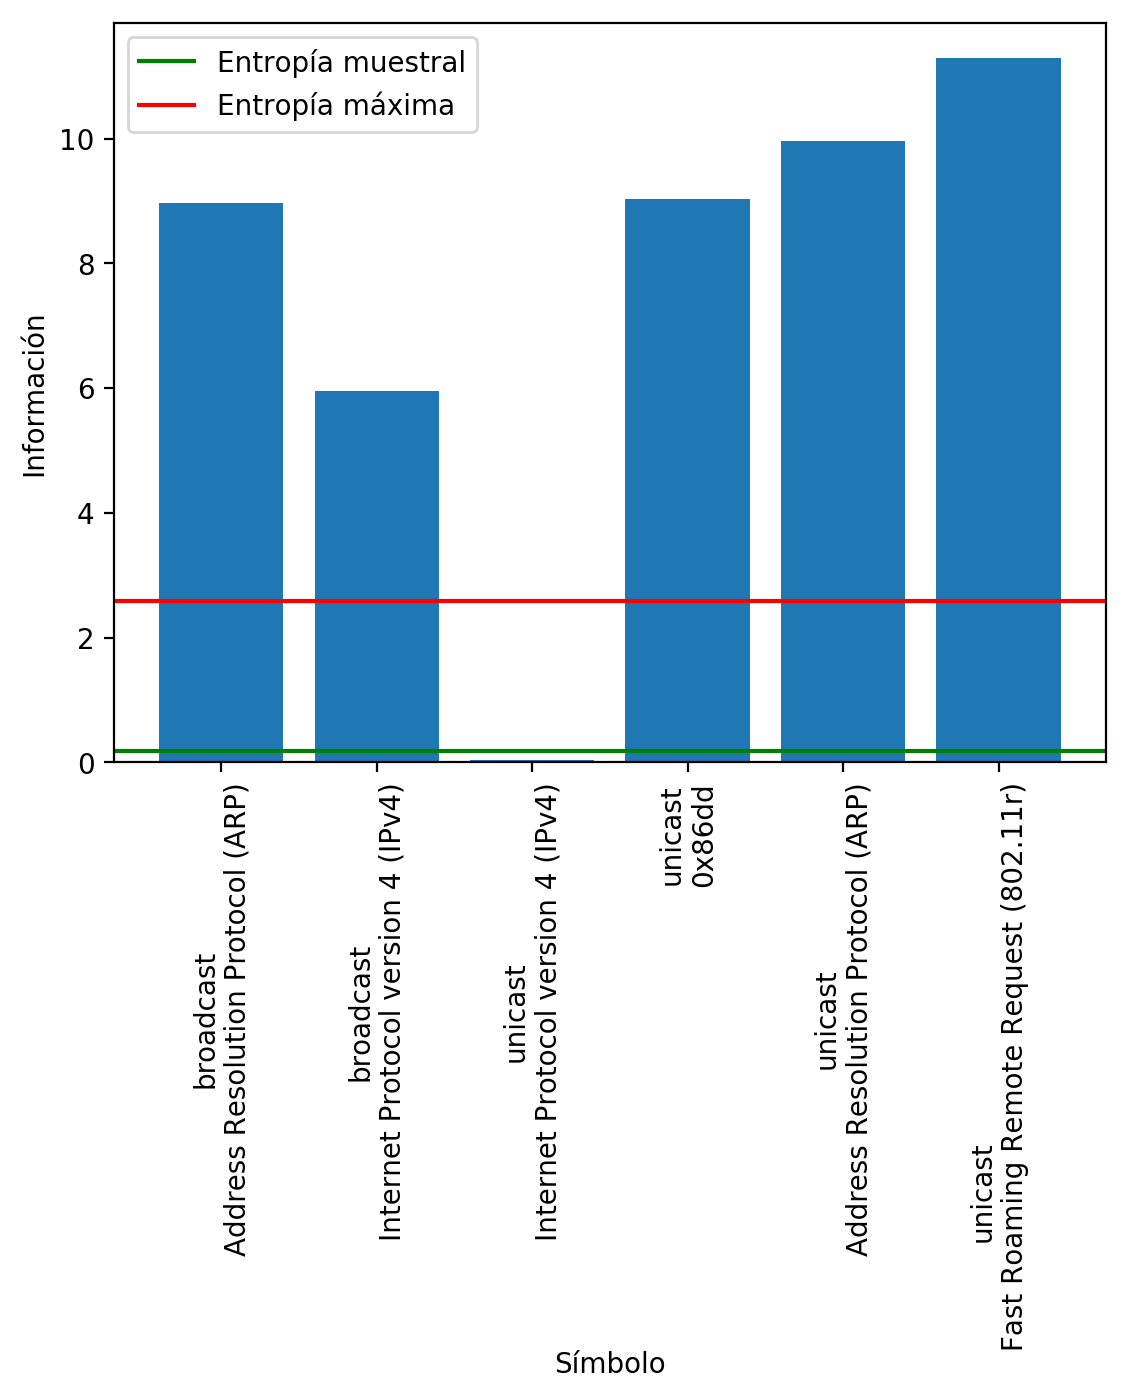
\includegraphics[width=0.7\textwidth]{entropiaS1Red2.png}
\caption{Gráfico de la información de los símbolos de la fuente $S_1$ observados en esta red. Se muestra la entropía muestral de $S_1$ y su entropía máxima.}
\label{entropias1_2}
\end{figure}

En el caso de la fuente $S_2$, como podemos ver en la figura 9, hay dos IPs particulares que aportan menos información que el resto. 
Se trata de las que envian requests de ARP con mas frecuencia. En este caso, al aportar todos los símbolos aproximadamente la misma información (comparativamente con la figura 8 donde hay un simbolo con muy poca informacion ) , la entropía muestral se encuentra cerca de la máxima.

\begin{figure}[H]
\centering
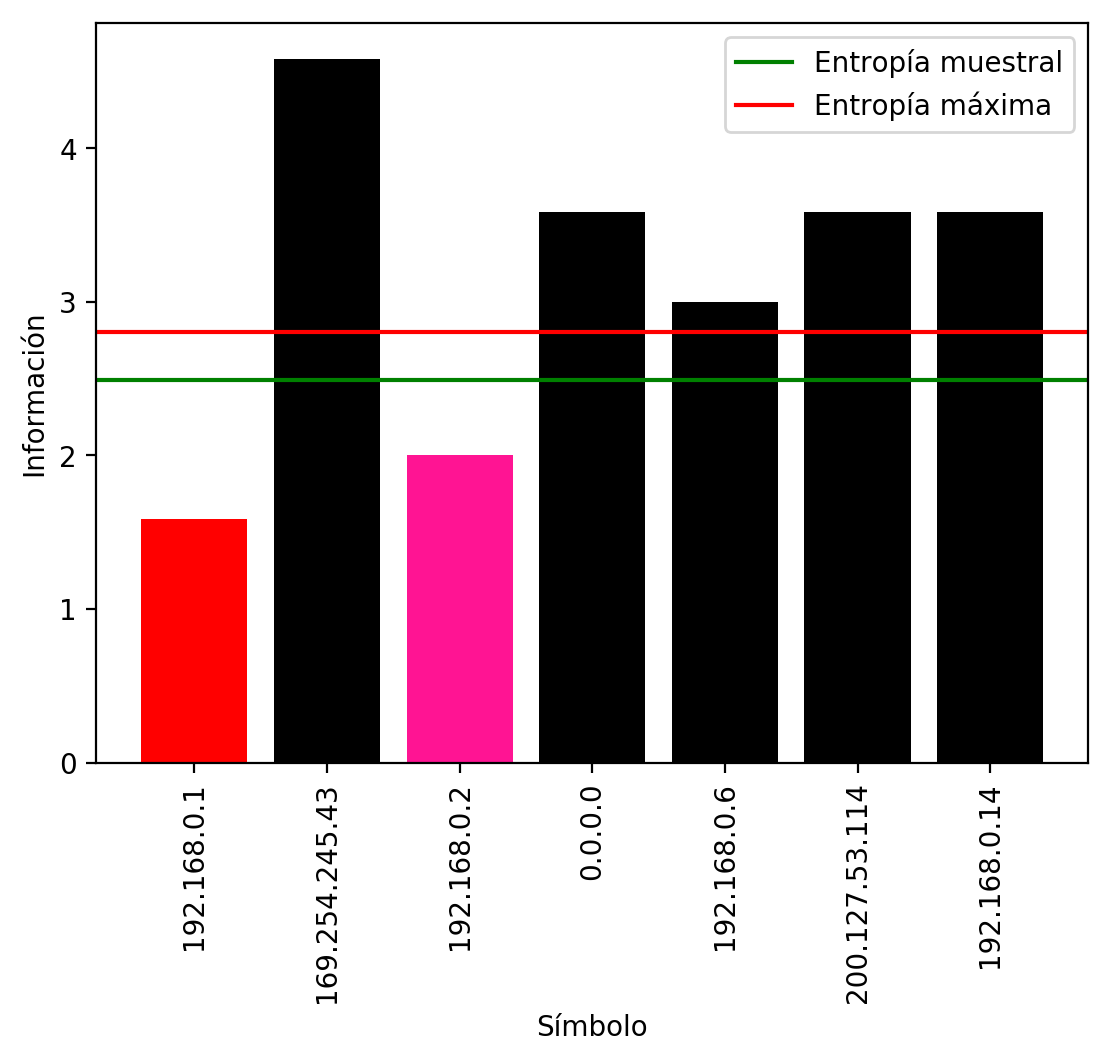
\includegraphics[width=0.7\textwidth]{entropiaS2Red2.png}
\caption{Gráfico de la información de los símbolos de la fuente $S_2$ observados en esta red. Se muestra la entropía muestral de $S_2$ y su entropía máxima.}
\label{entropias2_2}
\end{figure}

Graficamos la red subyacente de mensajes ARP en la figura~\ref{grafo2}. Los nodos representan a los hosts y las aristas los mensajes ARP de los dos tipos. 
Podemos ver que los nodos correspondientes a las dos IPs con menor informacion son las que tienen mayor grado en el grafo ( grado 4 para 192.168.0.1 y grado 3 para 192.168.0.2 )

\begin{figure}[H]
\centering
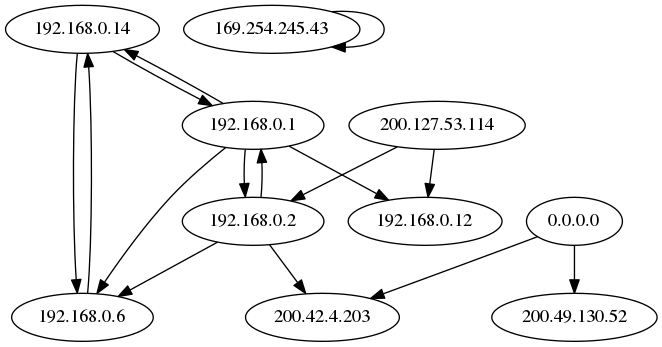
\includegraphics[width=0.7\textwidth]{grafoRed2.png}
\caption{Grafo de la red de mensajes ARP subyacente. Los nodos son las IPs observadas y los ejes son los mensajes ARP. En colores se marcan los nodos distinguidos (información por debajo de la entropía) y sus mensajes salientes. Cada arista tiene anotada la cantidad de requests/replies ARP.}
\label{grafo2}
\end{figure}